\section{Deelvraag 4: Requirements}
In dit hoofdstuk word de vierde deelvraag onderzocht \SubquestionFour.
Om met deze deelvraag te beantwoorden zijn er semi gestructureerde interviews gehouden met de product owner en de CEO van Snakeware.
Tijdens de interviews wordt er gepraat over de eisen en wensen zodat deze in kaart kunnen worden gebracht.
Bijde interviews zijn terug te vinden in bijlage \ref{appendix:ExploreUserRequirements}

\subsection{Interview product owner}
Het eerste interview wat plaats heeft gevonden is gedaan met de product owner Elsa Croes.
Om Elsa te ondersteunen en meer technisch beeld te schapen is er op het laatst een frontend developer mee genomen in het gesprek Eric Dijkstra.
Het interview heeft plaats gevonden op 6 november 2023 op locatie.
Tijdens het interview zijn er verschillende vragen gesteld om een beeld te krijgen van de toekomst visie van de applicatie.
Het complete interview is te vinden in bijlage \ref{appendix:ExploreUserRequirementsElsa}.
De complete lijst met de requirements die uit dit interview zijn te zien in \ref{fig:ElsaRequirements}.
Deze lijst is daarna aan Elsa Croes gentoont en heeft ze als goed beschoud.
\todo[inline]{Nog even terug leggen bij Elsa}

\whitespace
\begin{graphic}
    \captionsetup{type=figure}
    \caption{Elsa Croes Requirements}
    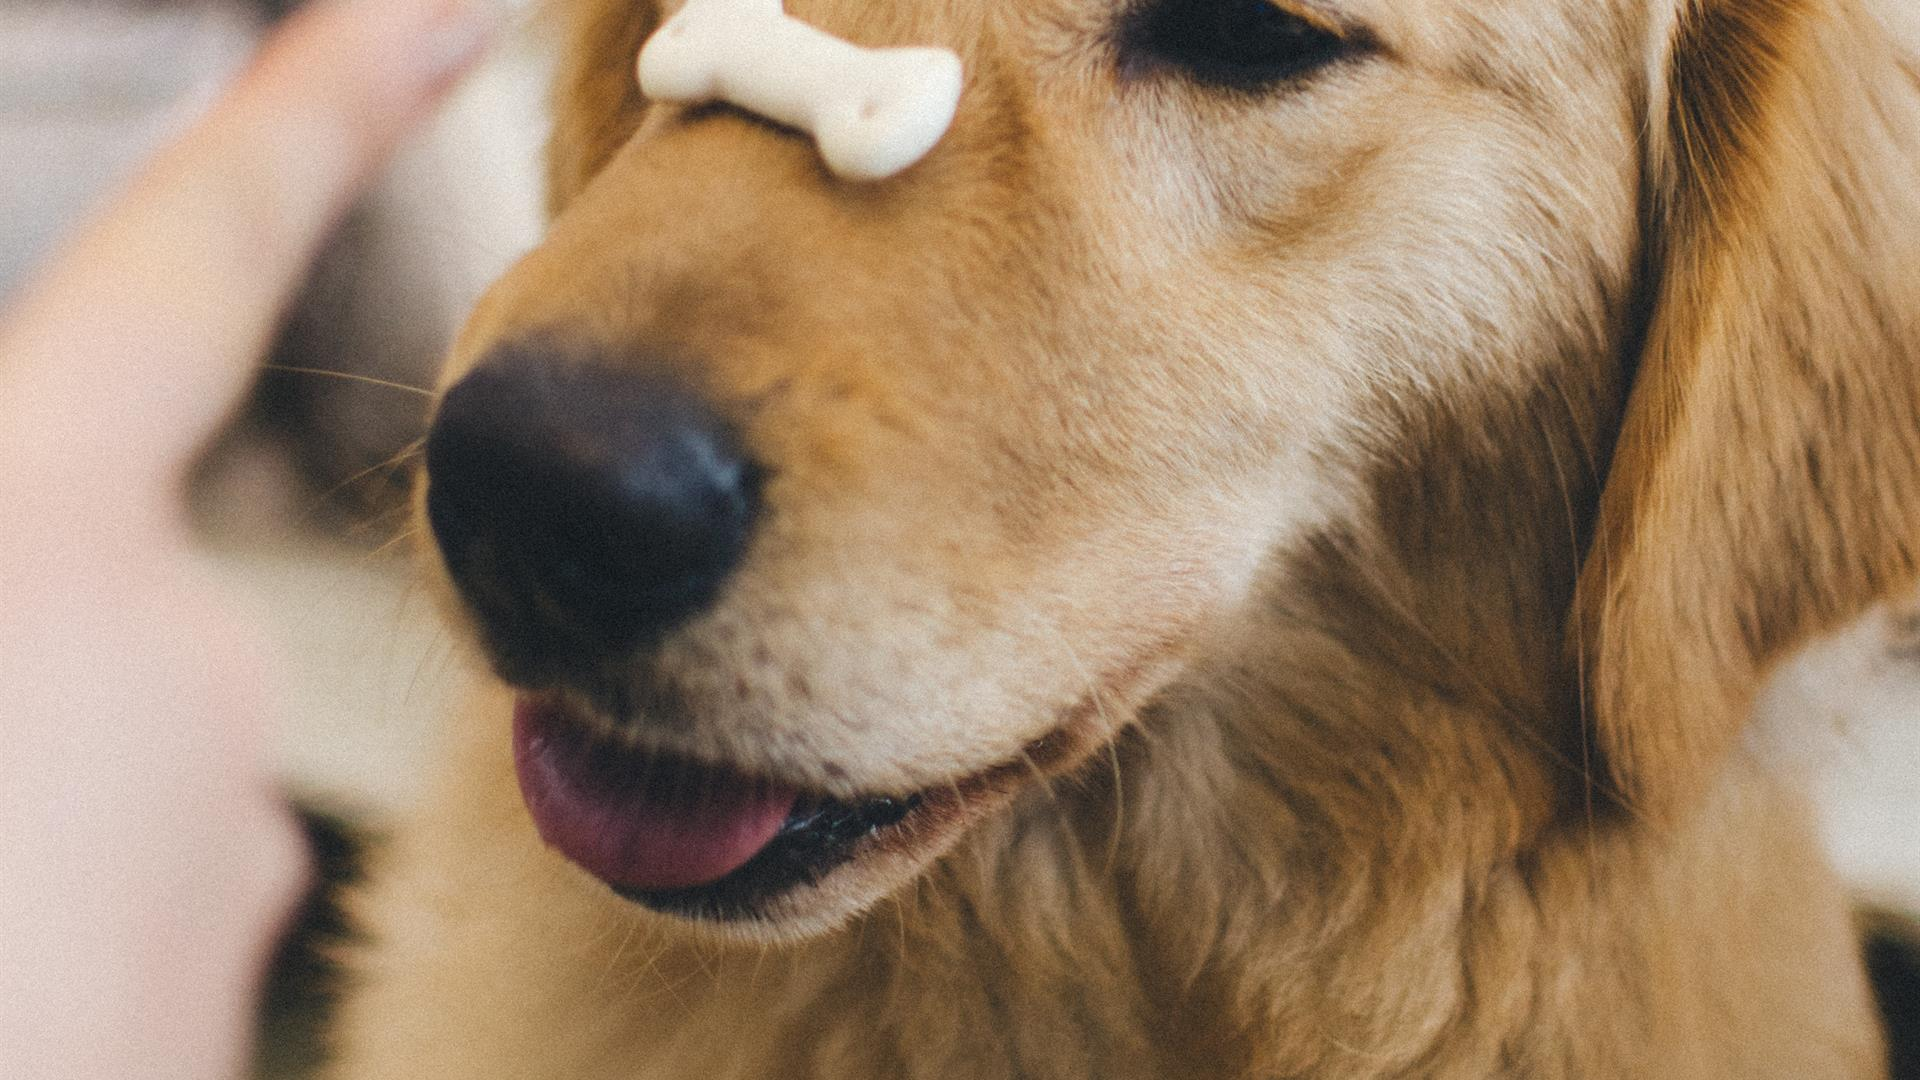
\includegraphics[scale=0.2]{Placeholder.jpg}
    \label{fig:ElsaRequirements}
\end{graphic}

\subsection{Interview CEO Snakware}
Dit interview is gedaan met Hans Hoomans CEO van Snakeware.
Het interview heeft plaats gevonden op 7 novemeber 2023 op locatie.
:w
\begin{graphic}
    \captionsetup{type=figure}
    \caption{Hans Hoomans Requirements}
    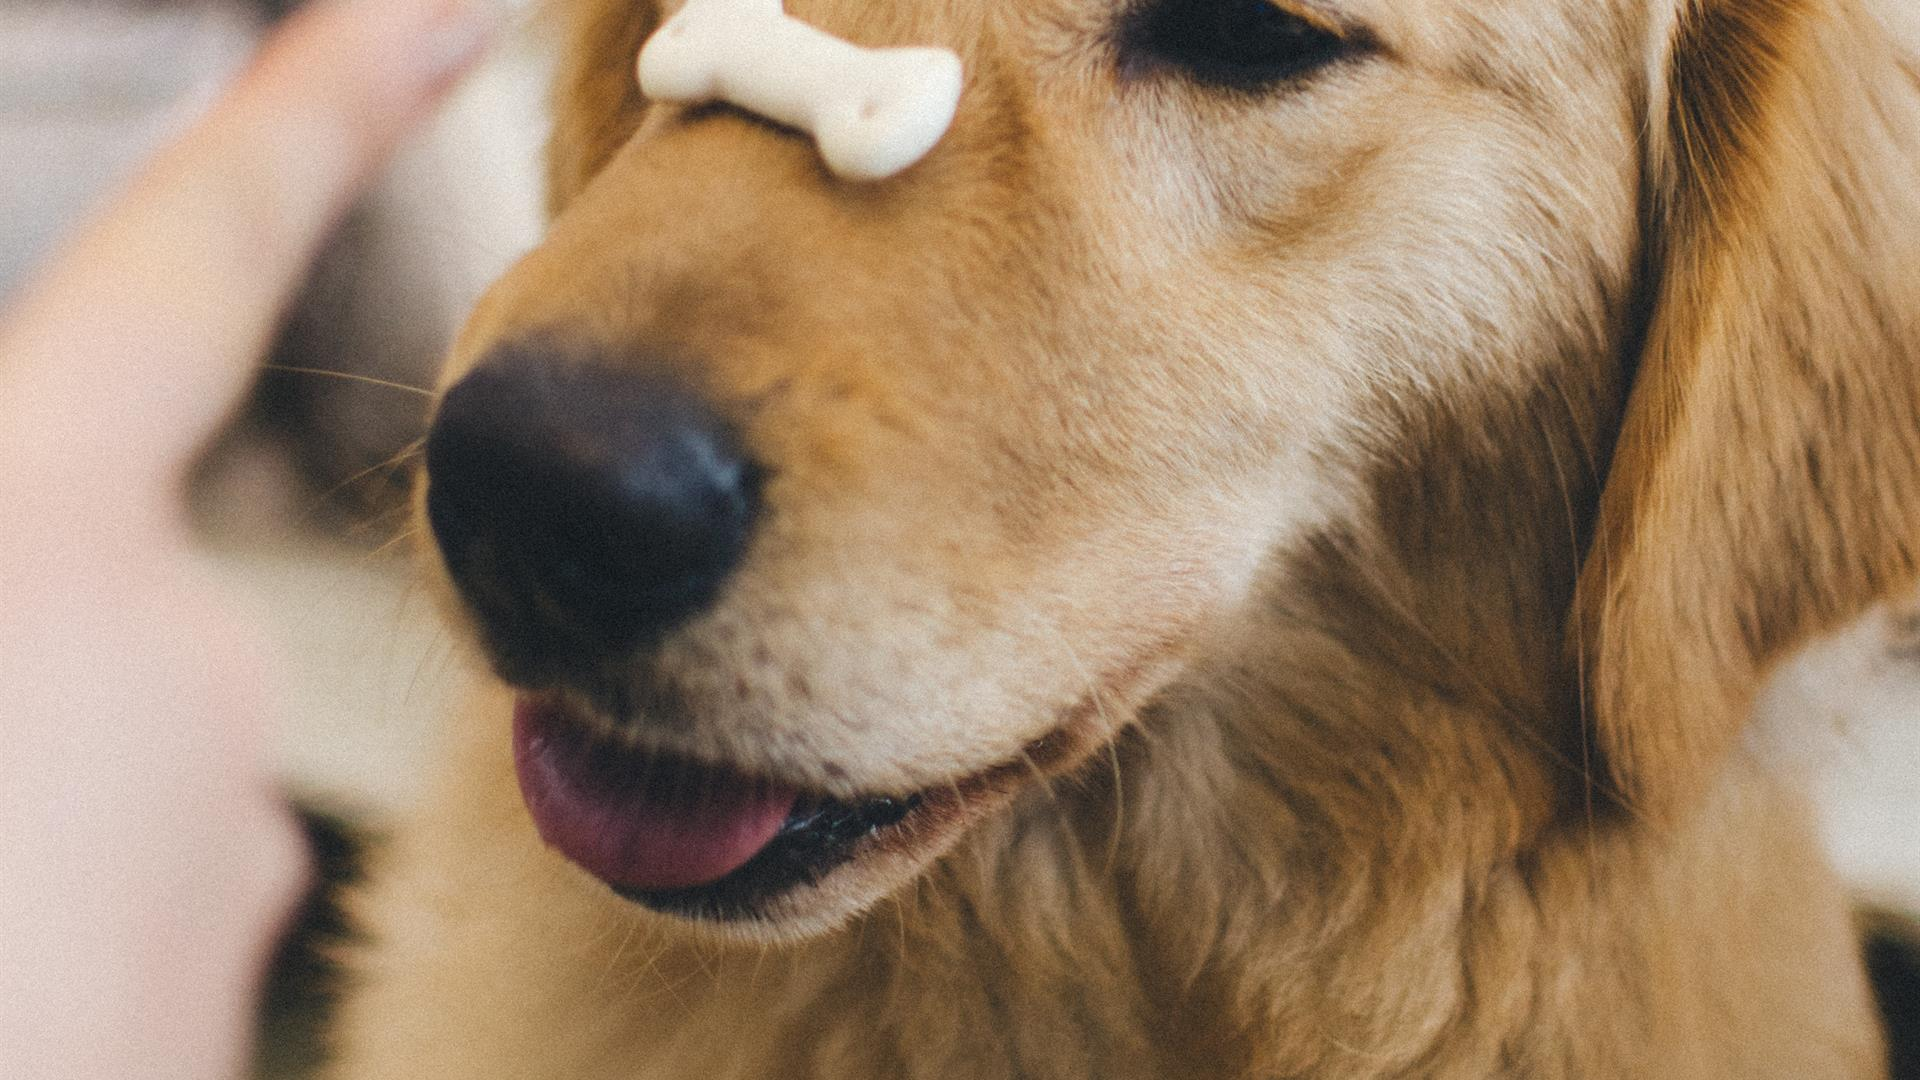
\includegraphics[scale=0.2]{Placeholder.jpg}
    \label{fig:HansRequirements}
\end{graphic}
